\subsection{Scripts}

Scripting is a way of automatically running a sequence of calculations.
A script is entered in the left-hand field of the Eigenmath window.

\begin{center}
\begin{tikzpicture}
\node at (0,0) {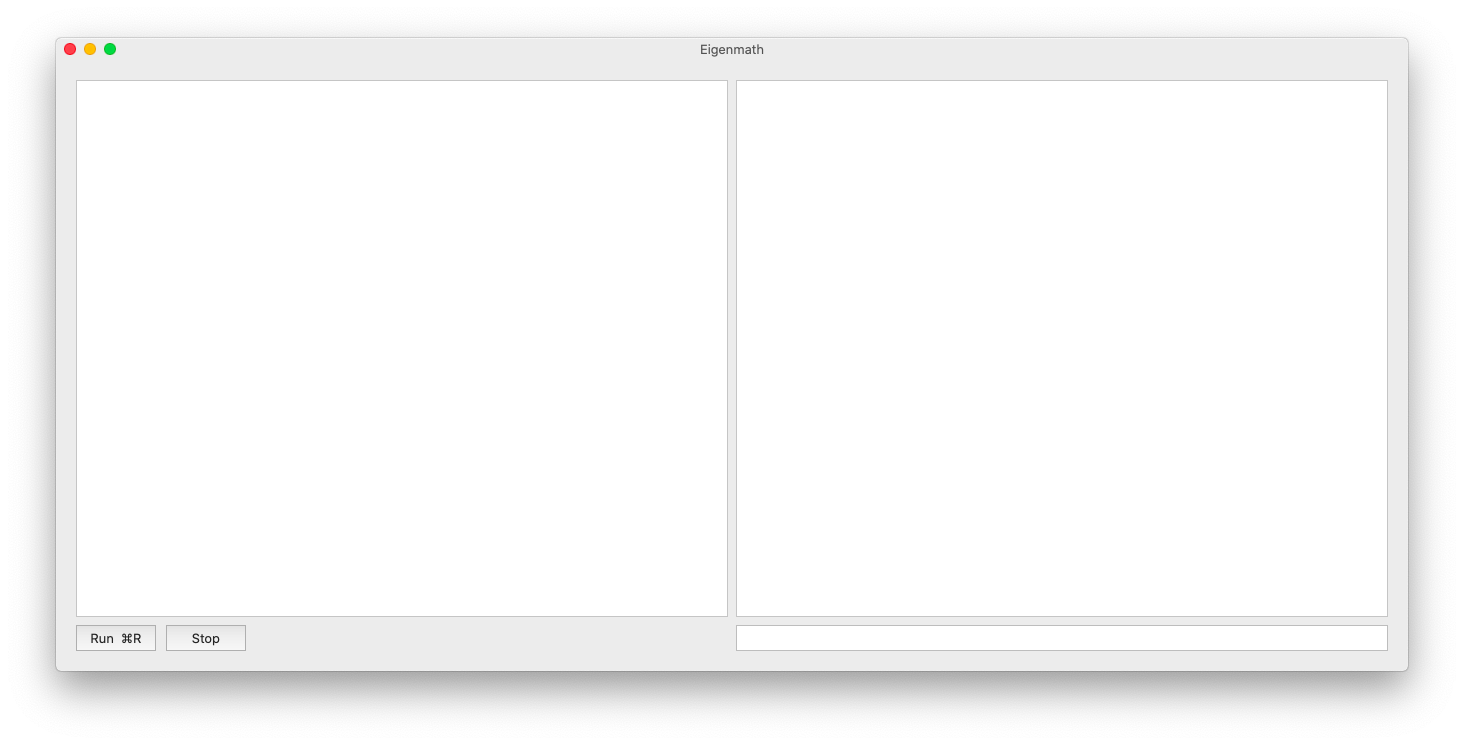
\includegraphics[scale=0.2]{face.png}};
\draw (-2.4,0.1) node {Scripts go here.};
\end{tikzpicture}
\end{center}

\noindent
To create a script, enter one calculation per line in the script field.
Nothing happens until the Run button is clicked. When the Run button is
clicked, Eigenmath evaluates the script line by line. After a script runs,
all of its symbols are available for immediate mode calculation.
Scripts can be saved and loaded using the File menu.

\bigskip
\noindent
Here is an example script that can be pasted into the script field
and then run by clicking the Run button.

\begin{Verbatim}[formatcom=\color{blue}]
"Solve for vector X in AX = B"
A = ((1,2),(3,4))
B = (5,6)
X = dot(inv(A),B)
X
\end{Verbatim}

\noindent
After clicking the Run button, the following result is displayed.

\bigskip
\noindent
\verb$Solve for vector X in AX = B$

\bigskip
\noindent
$\displaystyle X=\begin{bmatrix}-4\\ \frac{9}{2}\end{bmatrix}$

\bigskip
\noindent
A handy debugging aid is to include the line $trace=1$ in the script.
When $trace=1$ each line of the script is displayed as it is evaluated.
For example, here is the previous script with the addition of
$trace=1$.

\begin{Verbatim}[formatcom=\color{blue},samepage=true]
"Solve for vector X in AX = B"
trace = 1
A = ((1,2),(3,4))
B = (5,6)
X = dot(inv(A),B)
X
\end{Verbatim}

\noindent
The result is

\begin{Verbatim}
Solve for vector X in AX = B
A = ((1,2),(3,4))
B = (5,6)
X = dot(inv(A),B)
X
\end{Verbatim}

\noindent
$X=\begin{bmatrix}-4\\ \frac{9}{2}\end{bmatrix}$
